\cleardoublepage
\chapter{Cognitive Language Agents for Question Answering}
\label{ch:development}
\label{ch:chapter3}

In this section, we first present the datasets used in our evaluation study, followed by a description of the evaluation framework. This framework supports the development of both the baseline systems and the proposed cognitive language agents. The baseline results are further analyzed in \textit{Analyzing Retrieval Scaling in RAG Systems for Complex QA Benchmarks} \cite{RayoMosquera2025}, a study published as part of this broader research effort.

\section{Datasets}

To evaluate our language agents and baselines models, we use three  well-known benchmarks for the MHQA task, \textbf{HotpotQA} \cite{yang2018hotpotqa}, \textbf{2WikiMultiHopQA} \cite{ho-etal-2020-constructing}, and \textbf{MuSiQue} \cite{trivedi2021musique}. Although prior work has shown that \textbf{HotpotQA} does not always require genuine multi-hop reasoning, we include it to support comparison with prior work \cite{trivedi2021musique}.

\noindent All evaluations are performed on the development sets of these datasets, which offer a sufficient number of samples for statistically meaningful results. Following the setup proposed by Bernal et al. \cite{NEURIPS2024_6ddc001d}, we construct a corpus for each dataset by combining the annotated supporting passages with distractor passages. To maintain consistency across evaluations, only answerable questions are retained.

\noindent In addition to the MHQA benchmarks, we evaluate our systems on \textbf{LoCoMo}, a lesser-studied dataset designed for conversational QA \cite{maharana-etal-2024-evaluating}. For this work, we select a smaller subset consisting of 10 conversations. The questions include a mix of multi-hop, temporal, open-domain, and single-hop queries. As with the other datasets, non-answerable questions are excluded. Including LoCoMo allows us to test whether the proposed cognitive agent architectures remain effective in conversational QA scenarios that may be less demanding than standard MHQA tasks.

\noindent Table \ref{tab:dataset_stats} summarizes key statistics of these datasets. MuSiQue and 2WikiMultiHopQA are the most challenging among the selected datasets. Both were explicitly designed to enforce multi-step reasoning and reduce shortcut exploitation by LLMs, making them particularly well-suited for evaluating the reasoning capabilities of our language agents.

\begin{table}[h]
    \centering
    \begin{tabular}[\textwidth]{
        >{\raggedright\arraybackslash}p{2cm}  % Left-aligned and wrapped
        c
        >{\centering\arraybackslash}p{2.5cm}
        >{\centering\arraybackslash}p{2.5cm}
        c
    }
        \toprule
        \textbf{\scriptsize Dataset} &
        \textbf{\scriptsize \# Documents} &
        \textbf{\scriptsize Avg Doc Length (chars)} &
        \textbf{\scriptsize Avg Doc Length (tokens)} &
        \textbf{\scriptsize \# Questions} \\
        \midrule
        LoCoMo\textsuperscript{1} & 5,882 & 207.4 & 54.7 & 1,525 \\
        HotpotQA & 66,609 & 531.9 & 120.2 & 7,405 \\
        2Wiki & 56,680 & 430.8 & 104.1 & 12,576 \\
        MuSiQue & 21,100 & 474.2 & 106.3 & 2,417 \\
        \bottomrule
        \multicolumn{5}{p{14cm}}{\footnotesize \textsuperscript{1} A document corresponds to a single message within a conversation.} \\
    \end{tabular}
    \caption{Dataset statistics.}
    \label{tab:dataset_stats}
\end{table}


\section{Evaluation Framework}
\label{evaluation_framework_sec}

We developed an evaluation framework in Python 3.13, publicly available at \href{https://github.com/oyar99/LanguageAgentsQA}{Language Agents QA}, designed to streamline experimentation with the datasets and to facilitate the implementation of both simple RAG baselines and more advanced language agent architectures.

\noindent The framework supports two execution modes: prediction and evaluation. The \textit{orchestrator} is responsible for initiating the appropriate mode, initializing the dataset and agent, and executing the workflow. 

\noindent Each agent implementation must adhere to a common interface that defines two methods: \textit{index} and \textit{reason}. In the \textit{index} method, the agent receives the preprocessed dataset and executes any offline procedures. In the \textit{reason} method, the agent receives a question and must return an object containing the final answer, the list of documents consulted during reasoning, and additional metadata such as token usage. 

\begin{figure}[h]
    \centering
    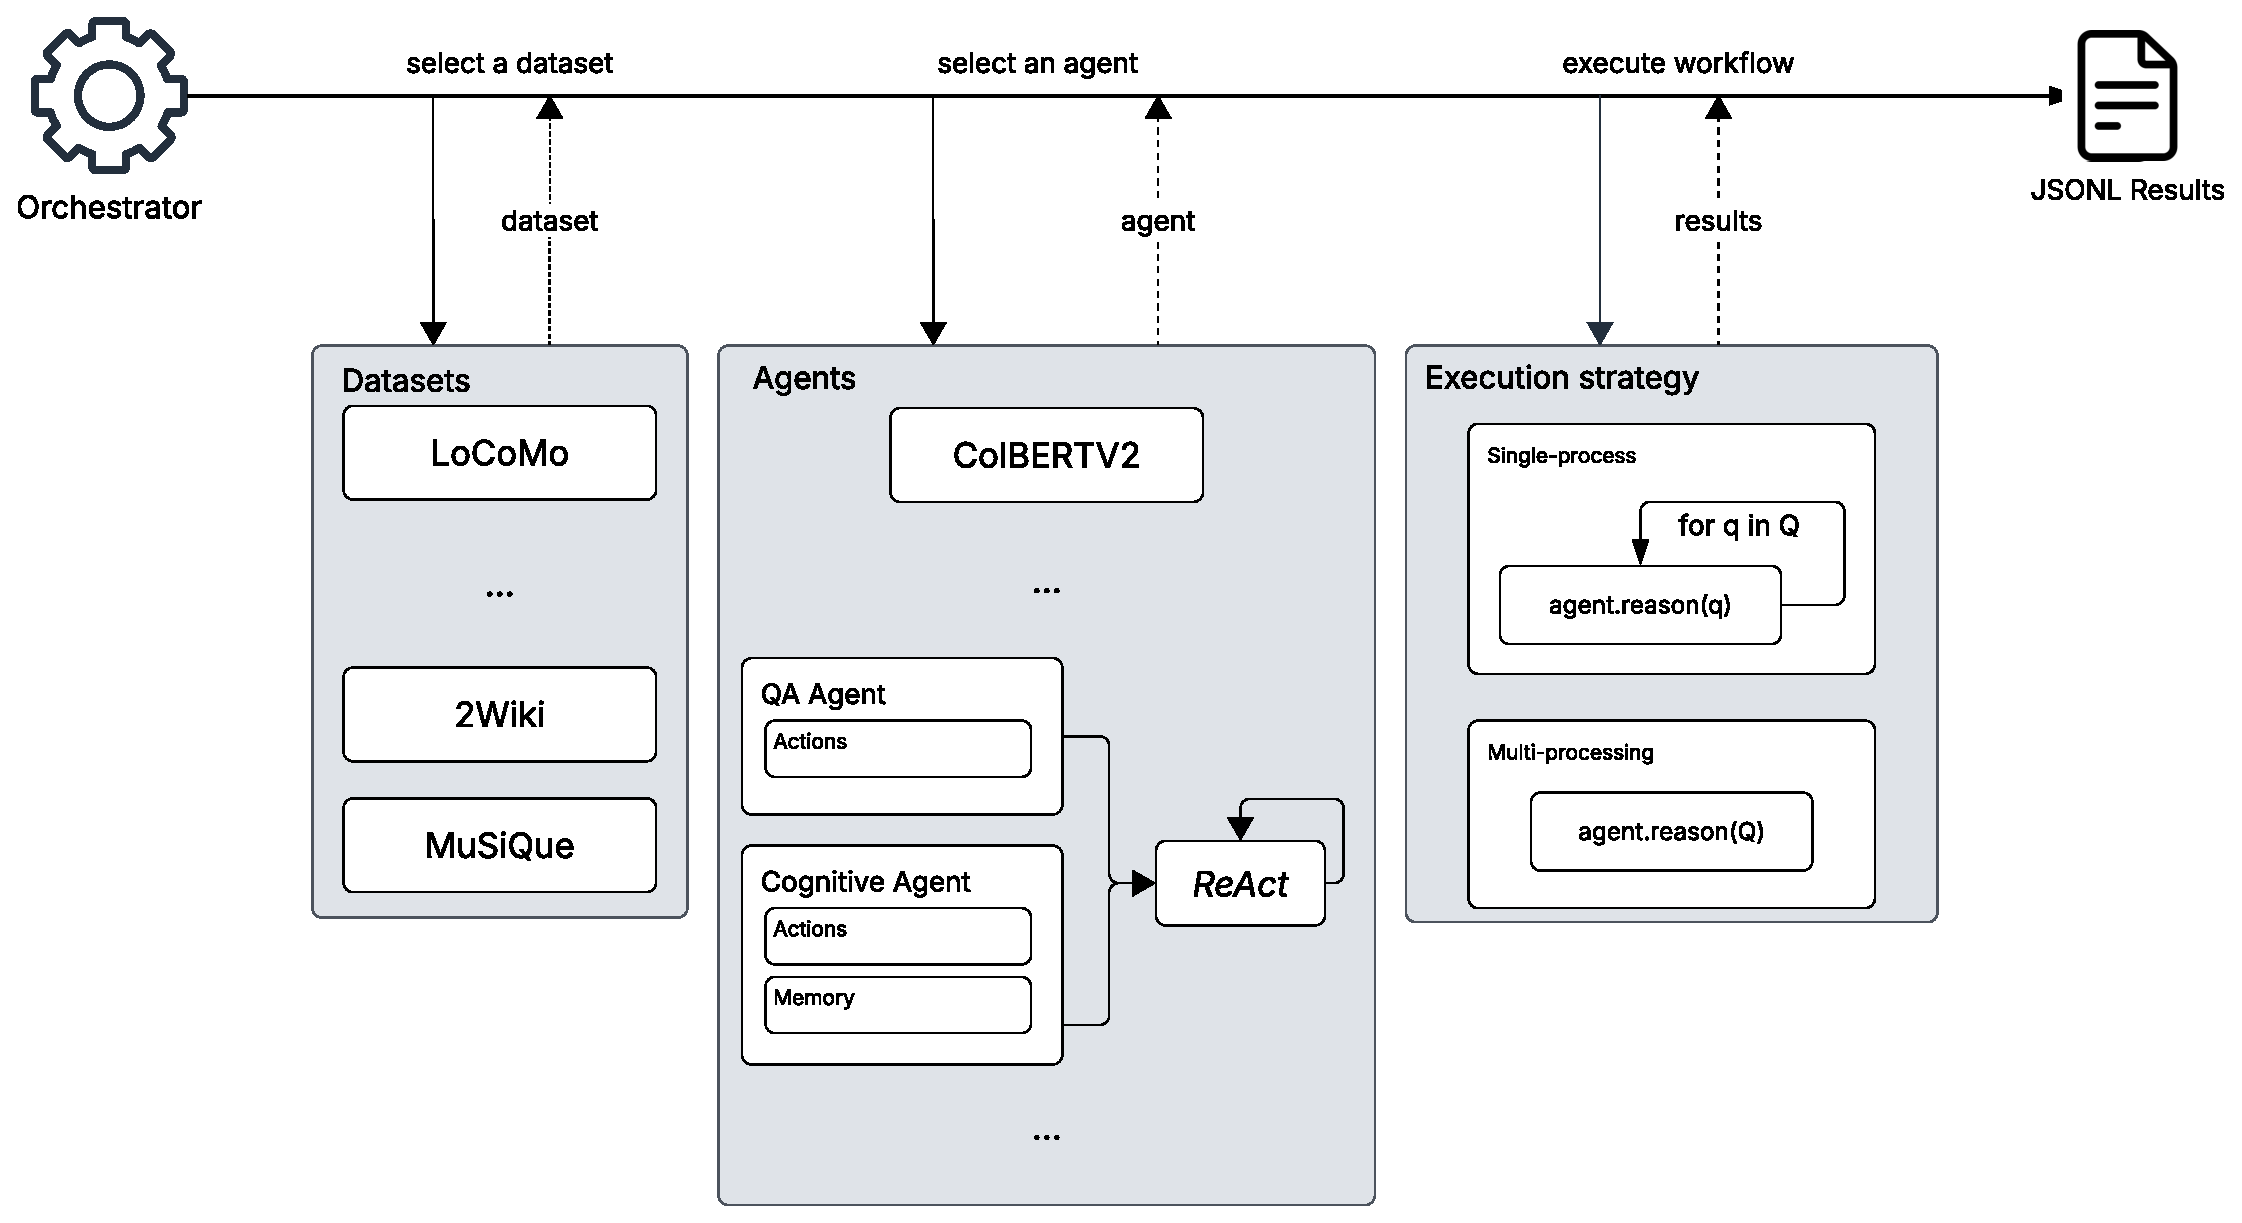
\includegraphics[width=1\textwidth]{images/eval-framework.eps}
    \caption{Evaluation framework architecture in prediction mode. The orchestrator (i) loads and initializes the dataset, (ii) configures the selected agent, and (iii) executes the question-answering workflow with the appropriate execution strategy.}
    \label{fig:eval_frame}
\end{figure}

\noindent The framework also provides a base implementation for more sophisticated agents. In particular, it includes an abstract ReAct agent that must be initialized with a set of actions. These actions, representing the agent's procedural memory, are Python functions paired with concise natural language descriptions. The base agent implements the ReAct reasoning loop following a structured well-defined JSON format. This implementation is designed for extensibility and can serve as the underlying reasoning engine for other agents. Importantly, the architecture is flexible enough to also implement baseline methods described in Section \ref{baselines_sec}, even when those methods are not strictly agent-based. An overview of the framework is provided in Figure \ref{fig:eval_frame}.

\noindent In evaluation mode, the script accepts a path to a JSONL file containing results and reports both retrieval and QA metrics, including recall, precision, $F_1$, recall@k, $EM$, $R_1$, $R_2$, and $L_1$.  

\noindent Furthermore, the framework supports multiprocessing, enabling independent processing of questions. In our experiments, we usually leverage up to 40 CPUs, substantially reducing execution time.

\noindent Finally, the framework integrates with vLLM, an inference and serving engine for LLMs. Any generative model available in vLLM can be used through the same interface as OpenAI's chat completions endpoint \cite{kwon2023efficient}.

\section{Baselines}
\label{baselines_sec}

We evaluated a range of retrieval systems, including both traditional lexical and semantic retrievers, as well as more advanced methods.

\noindent First, we used a BM25 ranking function with hyperparameters $b = 0.75$ and $k_1 = 0.5$. These values were selected experimentally, considering that passages across all four datasets are relatively short \cite{10.1145/2682862.2682863}. Both  documents and queries were processed through a standard normalization pipeline that includes unigram and bigram generation, stopword removal, Snowball stemming, and other text normalization techniques.

\noindent Second, we evaluated a semantic retriever based on the msmarco-bert-base-dot-v5 model, which encodes text into a 768-dimensional embedding space. This model, trained on question answer pairs from the MS Marco dataset, has demonstrated strong performance on a range of natural language tasks including QA \cite{reimers-2019-sentence-bert}.

\noindent Third, we included ColBERTv2, a semantic retriever that leverages contextual late interaction. Unlike single-vector dense retrievers, ColBERTv2 compares queries and documents at the token level, allowing for finer-grained relevance retrieval \cite{santhanam-etal-2022-colbertv2}.

\noindent To explore retrieval methods that leverage structured knowledge, we evaluated HippoRAG, a recent architecture inspired by neurobiological systems. HippoRAG constructs a knowledge graph by extracting triples from the corpus using an LLM. In our experiments, we used both QWen2.5-14B-Instruct and GPT-4o-mini \cite{qwen2}. HippoRAG also uses a dense embedding model during both indexing and QA \cite{NEURIPS2024_6ddc001d}, in our case Contriever \cite{lei-etal-2023-unsupervised}. This structured representation enables competitive performance, particularly on more challenging datasets such as MuSiQue.

\noindent To construct a strong baseline for these retrievers, we implemented several standard RAG systems, with carefully designed QA prompt templates to maximize question answering scores. (See Appendix \ref{ch:appendices}). For each system, we varied the number of retrieved passages $k$, from $5$ to $100$, to assess the impact of effective context length on performance. We also tested a FULL-CONTEXT variant in which all documents are provided to the model, ensuring that relevant ground-truth passages are always included, even if truncation is needed to fit within the model's context window. Due to computational constraints, questions in the FULL-CONTEXT setting are processed in batches of size 8, and the model is required to return structured outputs to locate the answer to each question deterministically. While this multitask scenario is not directly comparable with the RAG baselines, it offers useful insight into how model performance scales as more context is used.

\noindent The baselines used GPT-4o-mini (2024-07-18) with a context window of $128k$ tokens. We used the OpenAI API using version 2024-12-01-preview, utilizing both the chat completions and batch processing endpoints for cost efficiency.

\noindent We also report results obtained with QWen2.5-14B-Instruct, which supports a $32K$ token context window \cite{qwen2}. This model was executed using vLLM with 16-bit floating precision on two NVIDIA A40 GPUs, each with 46GB of VRAM \cite{kwon2023efficient}.

\noindent For a few scenarios, we additionally evaluated o3-mini (2025-01-31), which provides a $200k$ token context window. For this model, we selected the medium reasoning effort configuration.

\noindent All models were run with temperature set to $0$ to ensure outputs are as deterministic as possible, and frequency and presence penalties were also set to $0$. The maximum number of completion tokens was set to $500$, which we found sufficient, as most answers are brief. Additionally, we designated the newline character (\textbackslash n) as a stop token, since many models, particularly smaller ones, struggled to adhere to the output formatting instructions and often appended additional commentary.

\section{Cognitive Language Agents}
\label{agents_sec}

Building on the evaluation framework, we design several language agent architectures aimed at improving QA performance. These agent are compared against baseline approaches, providing an analysis of their effectiveness, including discussion on system complexity, performance trade-offs, and resource efficiency.

\begin{figure}[t]
    \centering
    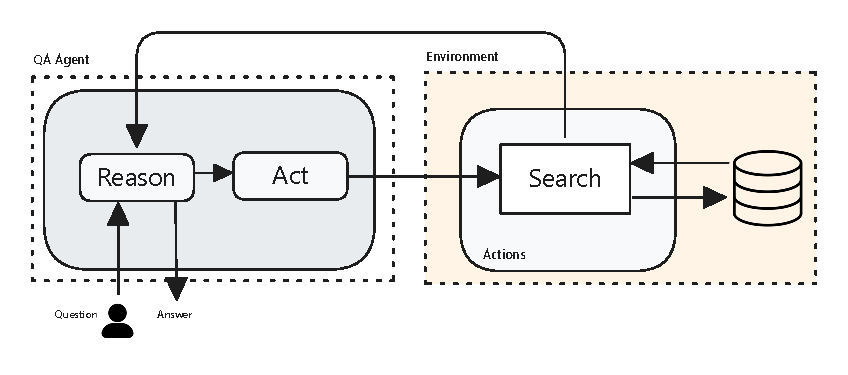
\includegraphics[width=1\textwidth]{images/qa_agent}
    \caption{QA Agent architecture using ReAct.}
    \label{fig:qa_agent}
\end{figure}

\noindent Agents grounded in the \textbf{ReAct} framework interleave reasoning and action. Actions typically correspond to search functions, and agents may also decompose complex questions into sub-questions to facilitate multi-step reasoning. The base prompt used to guide these agents is shown in Figure \ref{fig:agent_base_prompt}, and individual variants adapt it with specific tools, tool descriptions, or illustrative examples.

\subsection{QA Agent}
\label{sec:qa_agent}

\noindent A \textbf{ReAct} agent uses a language model $M$ to reason and interact with the environment, where a single single action is defined to retrieve relevant passages using a retriever $R$. Once sufficient context is gathered, the agent produces an answer. The agent uses 2-shot prompting to guide its reasoning and acting. The architecture is shown in Figure \ref{fig:qa_agent}.

\noindent In our experiments, we test with language model $M$, GPT-4o-mini, and retrievers $R$: ColBERTv2 and HippoRAG both retrieving 5 documents per query.

\noindent We implement minor variants to experiment introduced below.

\subsubsection{QA Agent with Re-ranking}

\noindent This agent introduces an LLM-based second-stage retriever that re-ranks the initial retrieval set. The retriever prioritizes higher-quality evidence and discards distractors before reasoning proceeds, thereby improving retrieval precision. The second-stage retriever is tested with GPT-4o-mini. The agent is shown in Figure \ref{fig:qa_reranking_agent}.

\begin{figure}[h]
    \centering
    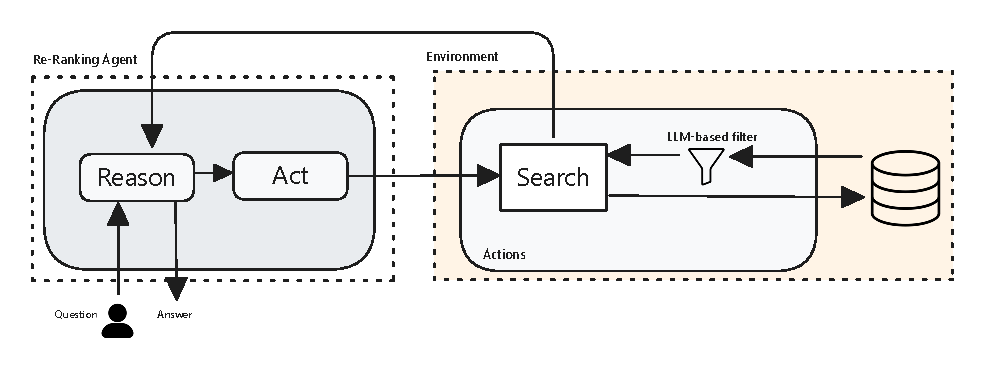
\includegraphics[width=1\textwidth]{images/reranking_agent.eps}
    \caption{QA Agent with re-ranking support.}
    \label{fig:qa_reranking_agent}
\end{figure}

\subsubsection{QA Agent with Pagination}

\noindent This variant augments the search tool of the QA agent by introducing a \textit{page} parameter, allowing the agent to retrieve additional results beyond the initial retrieval set. For example, calling \textit{search('northwestern Somalia', 2)} returns passages ranked from position 6 to 10. This mechanism enables exploration of a broader retrieval space when necessary.

\subsubsection{QA Agent with Self-Reflection}

\noindent This variant incorporates a reflection mechanism that enables the agent to recognize when it is not making meaningful progress toward an answer. The agent records its ongoing reasoning steps in a separate episodic memory. After each reasoning iteration, it evaluates whether the last $m$ thoughts have led to useful progress. If not, the agent pauses to analyze the retrieved observations to make inferences and formulate a new plan of action. Although simple, this mechanism helps redirect the agent's trajectory and maintain focus on the question.

\subsection{DAG Agent}

\noindent We take inspiration on frameworks such as \textit{PAR RAG} \cite{zhang2025credibleplandrivenragmethod} and \textit{Plan-and-Solve} \cite{wang-etal-2023-plan} to design an agent that begins by constructing a plan in the form of a Directed Acyclic Graph (DAG). This is achieved by explicitly prompting a language model $M$ to build a graph $G$ that identifies sub-questions and clearly defines the order in which they must be answered.

\noindent Once the DAG is constructed, we define an execution loop that runs up to $T$ times or until all nodes in the graph are completed. At each iteration, the loop selects nodes with no incoming edges, sub-questions without unresolved dependencies, and prompts $M$ to solve them. Nodes can be of two types: (i) inference questions, whose answers can be derived from completed dependencies, or (ii) retrieval questions, which require additional information. For the latter, the model executes an \textit{ANSWER} function $A(q)$ that returns a tuple consisting of the answer, a reasoning trace, and the retrieved documents for query $q$. If $A(q)$ yields a valid answer, the node is marked as \textit{completed} and annotated with the trace and documents. Otherwise, it is marked as \textit{failed}.

\noindent When a node fails, the agent attempts to backtrack. It traverses upward to ancestor nodes and prompts $M$ to propose alternative answers based on the documents attached to those nodes. If plausible alternatives are found, all descendant nodes are reset and the exploration restarts. If no alternatives are found, the ancestor node is restored to its original completed state. Each of these recovery attempts is recorded in the reasoning trace. Once no more alternatives exist for a node, it is marked as \textit{exhausted}, and backtracking continues until either new alternatives are found or we reach a node with no dependencies, at which point the loop eventually exits.

\noindent When the execution loop terminates, either because it has been forcibly exited or all nodes have been successfully completed, the model $M$ synthesizes a final answer based on the state of $G$. In cases where $G$ contains failed nodes, the de-serialized structure includes the failed nodes documents, though dependencies may be incomplete, limiting the chance of a correct final answer.

\noindent This procedure is formalized in Algorithm \ref{alg:qa-dag}, which details the planning, execution, and synthesis phases of the agent. 

\begin{algorithm}[H]
\caption{QA DAG Agent Reasoning Procedure}
\label{alg:qa-dag}
\KwIn{Question $q$}
\KwOut{Final answer $a$ and documents $\Sigma(v)$}

\BlankLine
\textbf{Phase 1: DAG Planning} \\
$G=(V,E) \gets M(\texttt{plan}(q))$ \tcp*{LLM produces DAG of sub-questions $v \in V$ with dependencies $E$}

\BlankLine
\textbf{Phase 2: Execution Loop} \\
$t \gets 0$\; 
\ForEach{$v \in V$}{
    $\text{ans}(v) \gets \emptyset$ \tcp*{answer of $v$}
    $\tau(v) \gets \emptyset$ \tcp*{reasoning traces for $v$}
    $\Sigma(v) \gets \emptyset$ \tcp*{supporting documents for $v$}
    $\text{original\_ans}(v) \gets \emptyset$ \tcp*{first non-empty answer of $v$}
}
$U \gets \{ v \in V \mid v \text{ has no incoming edges} \}$\;

\While{$t < T \ \text{and } U \neq \emptyset$}{
    $\text{restart} \gets \text{false}$\;
    \ForEach{$u \in U$}{
        \uIf{$u$ is \textbf{inference}}{
            $\text{ans}(u) \gets M(\texttt{answer}(u))$
        }
        \uElseIf{$u$ is \textbf{retrieval}}{
            $(\text{ans}(u),\; \tau(u),\; \Sigma(u)) \gets A(u)$\;
        }

        $\text{original\_ans}(c) \gets \text{ans}(c)$\;
        
        \uIf{$\text{ans}(u) = \emptyset$}{  % node failed
            % --- build ordered ancestor candidates (closest ancestors first)
            $\text{Candidates} \gets \mathrm{sort}_{\uparrow\!\mathrm{dist}}\big(\text{Ancestors}(u)\big)$\;
            \ForEach{$c \in \text{Candidates}$}{
                \If{$\neg\text{exhausted}(c)$}{
                    $\text{Alt} \gets M(\texttt{revise}(c))$\;
                    \If{$\text{Alt} \neq \emptyset$}{
                        $\text{ans}(c) \gets \text{Alt}$\;
                        \ForEach{$v \in \text{Descendants}(c)$}{
                            $\text{ans}(v) \gets \emptyset,\; \tau(v) \gets \emptyset,\;$
                        }
                        $\text{restart} \gets \text{true}$\;
                        \textbf{break} % break Candidates loop
                    }
                    \uElse{
                        $exhausted(c) \gets \text{true}$\;
$\text{ans}(c) \gets \text{original\_ans}(c)$
                    }
                }
            }
            \If{$\text{restart}$}{ \textbf{break} } % break U loop to restart execution
        }
    } % end for each u in U

    % recompute executable set and advance iteration
    $U \gets \{ v \in V \mid \text{ans}(v) = \emptyset \ \text{and } \forall (u,v)\in E,\; \text{ans}(u) \neq \emptyset \}$\;
    $t \gets t + 1$\;
}

\BlankLine
\textbf{Phase 3: Answer Synthesis} \\
$a \gets M(\texttt{synthesize}(\{\text{ans}(v),\tau(v)\}_{v\in V}))$\;

\BlankLine
\Return $a$ and $\Sigma(\cdot)$\;

\end{algorithm}


\noindent The DAG itself serves as the agent's episodic memory, storing sub-questions, reasoning traces, answers, and retrieved documents. Unlike frameworks such as ReAct, which make it difficult to detect reasoning or retrieval errors during execution, our approach leverages a programmatically assisted procedure that deterministically identifies and recovers from such errors. 

\noindent Our backtracking mechanism can be interpreted as a form of reflection, where the agent revisits ancestor nodes and evaluates plausible alternatives within a bounded search space, enabling the agent to correct earlier missteps in a controlled manner.

\noindent For example, our approach correctly identifies expected answers in cases involving conflicting information. Consider the MuSiQue question \textit{Who is the spouse of the Green performer?}, for which the model generates the plan illustrated in Figure \ref{fig:dag_example}.

\begin{figure}[h]
    \centering
    \lstinputlisting{./chapter3/dag_example.txt}
    \caption{DAG plan generated for question \textit{Who is the spouse of the Green performer?}.}
    \label{fig:dag_example}
\end{figure}

\noindent When the agent attempts to solve sub-question $node_1$, it retrieves the following documents.

\begin{quote}
    - \textit{Chuck Green}: "Chuck Green" (November 6, 1919 - March 7, 1997) was an American tap dancer.\\
    - \textit{Green (Steve Hillage album)}: Green is the fourth studio album by British progressive rock musician Steve Hillage.
\end{quote}

\noindent Initially, the agent selects the first document and answers \textit{Chuck Green}. However, when addressing $node_2$, it fails to find information about Chuck Green's spouse, since that information is not available in the corpus. At this point, the agent backtracks, recognizes that an alternative answer (\textit{Steve Hillage, performer of the album Green}) is plausible, and resumes execution. This correction ultimately leads the agent to the expected answer \textit{MiQuette Giraudy}.

\noindent Similarly, our approach is effective when prior knowledge biases the agent toward an incorrect path. Consider the HotpotQA question \textit{In what year was the writer of The Bet born?}. The retriever obtains the following document.

\begin{quote}
    The Bet is a 1992 American short film directed by Ted Demme, written by Gavin O'Connor, and starring Josh Mosby and John B. Hickey.
\end{quote}

\noindent Here, the agent may incorrectly assume that the question refers to \textit{Anton Checkhov's} 1889 short story \textit{The Bet}, since this story is more widely known and likely appears more frequently in the training data. This initial bias can prevent consideration of alternative interpretations. Our backtracking procedure enables the agent to revisit this assumption, recognize that the necessary information about Chekhov is absent, and instead recover the intended answer by shifting to the 1992 film context.

\noindent In our experiments we use GPT-4o-mini and GPT-4.1-mini as the language model $M$. The function $A(q)$ is implemented using the QA Agent introduced in Section \ref{sec:qa_agent}, with ColBERTv2 as the retriever and GPT-4o-mini as the language model. This architecture furthers allows decoupling reasoning and execution, where larger models can be used for generating the DAG or synthesizing answers, while smaller models handle sub-question solving, a flexibility not easily achieved with ReAct-style agents.

\subsubsection{Autonomous DAG Agent}

We also explore an alternative implementation of the execution loop in Algorithm \ref{alg:qa-dag}, where the entire process is delegated to a ReAct-style agent. Instead of a programatically orchestrated loop, the agent autonomously controls execution through two tools.

\begin{itemize}
    \item[] $answer(query: str, node\_id: str)$: calls the function $A(q)$ to obtain an answer for a sub-question. It returns the updated node state, including the answer and supporting documents. If $A(q)$ fails to produce an answer, the tool returns verbatim feedback prompting the agent to generate alternative answers for an ancestor node.
    \item[] $update\_node(value: str, node\_id: str)$: updates the answer of the specified node, resetting all descendant nodes if they were previously completed. This tool also returns feedback recommending the next steps.
\end{itemize}

\noindent With these tools, the agent learns to both advance through the DAG and backtrack when necessary. This allows it to reflect on prior decisions, recover from failures, and maintain coherence through verbal reinforcement learning.

\noindent Note that in later sections, we refer to this variant as the \textit{Auto DAG Agent}.

\subsection{Cognitive Agent}

\noindent We propose a cognitive language agent that incorporates episodic memory to store information about the questions it has answered during its lifetime. Unlike the previously described agents, this agent lifetime extends beyond a single QA session. The memory schema is shown in Figure \ref{fig:mem-schema}.

\begin{figure}[!htbp]
    \centering
    \lstinputlisting{./chapter3/cognitive_agent_memory_schema.txt}
    \caption{Long-term memory schema.}
    \label{fig:mem-schema}
\end{figure}

\noindent Like the previous agents, it follows a ReAct loop, but with one key distinction, after generating an answer, the agent evaluates it against the ground truth, simulating a human-in-the-loop process. If the answer is correct, the reasoning trace is stored directly in memory. Otherwise, the agent reflects on the error, reconstructs a reasoning trace that would have led to the correct answer, and stores that instead.

\begin{figure}[!htbp]
    \centering
    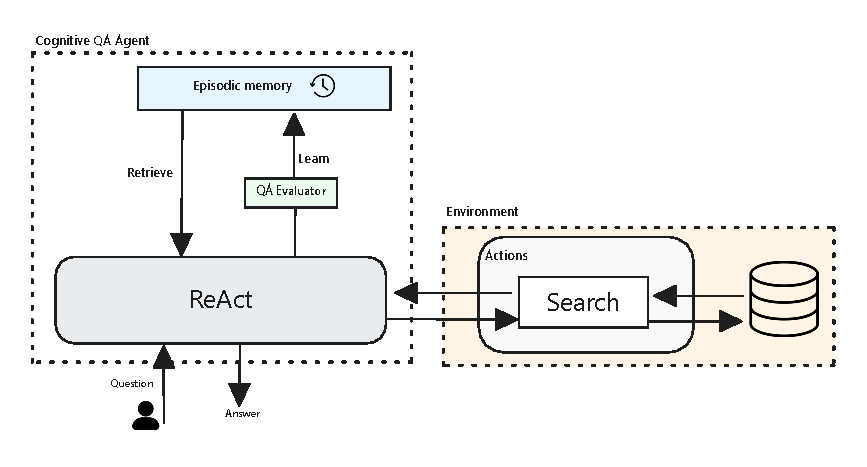
\includegraphics[width=1\textwidth]{images/cognitive_agent.eps}
    \caption{Cognitive Agent architecture.}
    \label{fig:cognitive_agent}
\end{figure}

\noindent An example of this reasoning trace format is provided in Figure \ref{fig:reasoning_chain}. When the agent is presented with a new question, it searches for up to $4$ semantically similar questions it has processed before using all-MiniLM-L6-v2, an embedding model that maps text to a 384-dimensional space \cite{reimers-2019-sentence-bert}. It then uses these questions as context for the current question. Over time, this architecture allows the agent to learn from experience and improve its performance, particularly on questions similar to those it has encountered before. Figure \ref{fig:cognitive_agent} illustrates the overall workflow.

\begin{figure}[h]
    \centering
    \lstinputlisting{./chapter3/reasoning_chain_sample.txt}
    \caption{Reasoning traces for question \textit{Because Marc Shiller was born in Beunos Aires in 1957, but is a resident of the United States, what ethnic group does he belong to?}}
    \label{fig:reasoning_chain}
\end{figure}

\begin{figure}[!htbp]
    \centering
    \lstinputlisting{./chapter3/prompt_base_agent.txt}
    \caption{ReAct agent prompt.}
    \label{fig:agent_base_prompt}
\end{figure}